\section{Setup}
\label{sec:setup}

\subsection{Test Environment}
\label{subsec:test_enviroment}

Figure~\ref{fig:campus_topo} presents the test environment used to evaluate IPro. This environment includes the campus network topology of the Federal University of Rio Grande do Sul \cite{isolani_2015:interactive}, the Ryu Controller, and the IPro prototype (\textit{cf.} Section ~\ref{subsec:prototype}). The monitored topology includes $11$ OpenFlow switches (version 1.3) that connect $230$ hosts from 7 laboratories (with 20, 30, and 40 hosts) and 4 administration offices (each one with 10 hosts) through links with a bandwidth of 10 Mbps each one. Furthermore, such topology includes a Web Server and a File Server connected in one of the administration offices. Each switch of the network is connected via a dedicated TCP channel to a remote Ryu controller used to coordinate network-wide forwarding decisions. The Mininet emulator \cite{lantz_2010:mininet} was used to deploy the monitored topology, which runs on a Ubuntu server with an Intel i7-4770 2.26 GHz and 8GB RAM. The Ryu Controller runs on a Ubuntu server with a Core i7-4770 processor and 2GB RAM.

\begin{figure}[H]
    \centering
    \includegraphics[width=0.75\columnwidth]{figures/Fig4-topology}
    \caption{Test Environment}
    \label{fig:campus_topo}
\end{figure}

To reliably test IPro, a realistic evaluation framework reflecting current and forecasted traffic patterns (\textit{e.g.,} web, P2P, and video) was used. In this master dissertation, to two measurement studies that investigate the composition of realistic traffic patterns \cite{labovitz_2011:interdomain, maier_2009:dominant} was resorted. The results indicate the dominance of Web traffic, amounting to 52\% overall measured traffic, followed by video traffic with 25-40\% of all traffic, while P2P traffic constituting only 18.3\% of total traffic. Thus, in all experiments, only Video and Web traffic was generated, in a proportion of 75\% to 25\%, respectively.\\

The Video traffic was generated by using the VLC media player \cite{Muller:2011:VMP:2072298.2072429} that can be used as a server and as a client to stream and receive video streams. The Web traffic was generated by using the Apache Server \cite{Mockus:2000:CSO:337180.337209} and http-clients based on Linux wget. These servers and clients were included in the campus topology. In this evaluation was assumed that all 230 hosts are active during the whole experiment time and place a request on average every 30 seconds. Furthermore, all experiment results have a confidence level equal to or higher than 95\%.
\subsection{Prototype}
\label{subsec:prototype}

Figure~\ref{fig:prototype_ipro} depicts the IPro prototype including: \textit{RL-agent}, \textit{Data Processing}, \textit{Flow Statistics Collection}, \textit{Data Repository}, \textit{Probing Manager}, \textit{Query Manager}, and \textit{Statistics Module}. \textit{RL-agent} and \textit{Data Processing} were developed and deployed using version 1.15 of Numpy that is the fundamental Python package for scientific computing. \textit{Probing Manager}, \textit{Query Manager}, and \textit{Statistics Module} were developed using the REST-based API provided by Ryu. This API helps to retrieve the switch statistics. \textit{Flow Statistics Collection} was developed using the Ryu API based on Python. \textit{Data Repository} was developed in MySQL. The IPRo prototype (including all test scripts) is available in \cite{castillo:ipro}.

\begin{figure}[H]
    \centering
    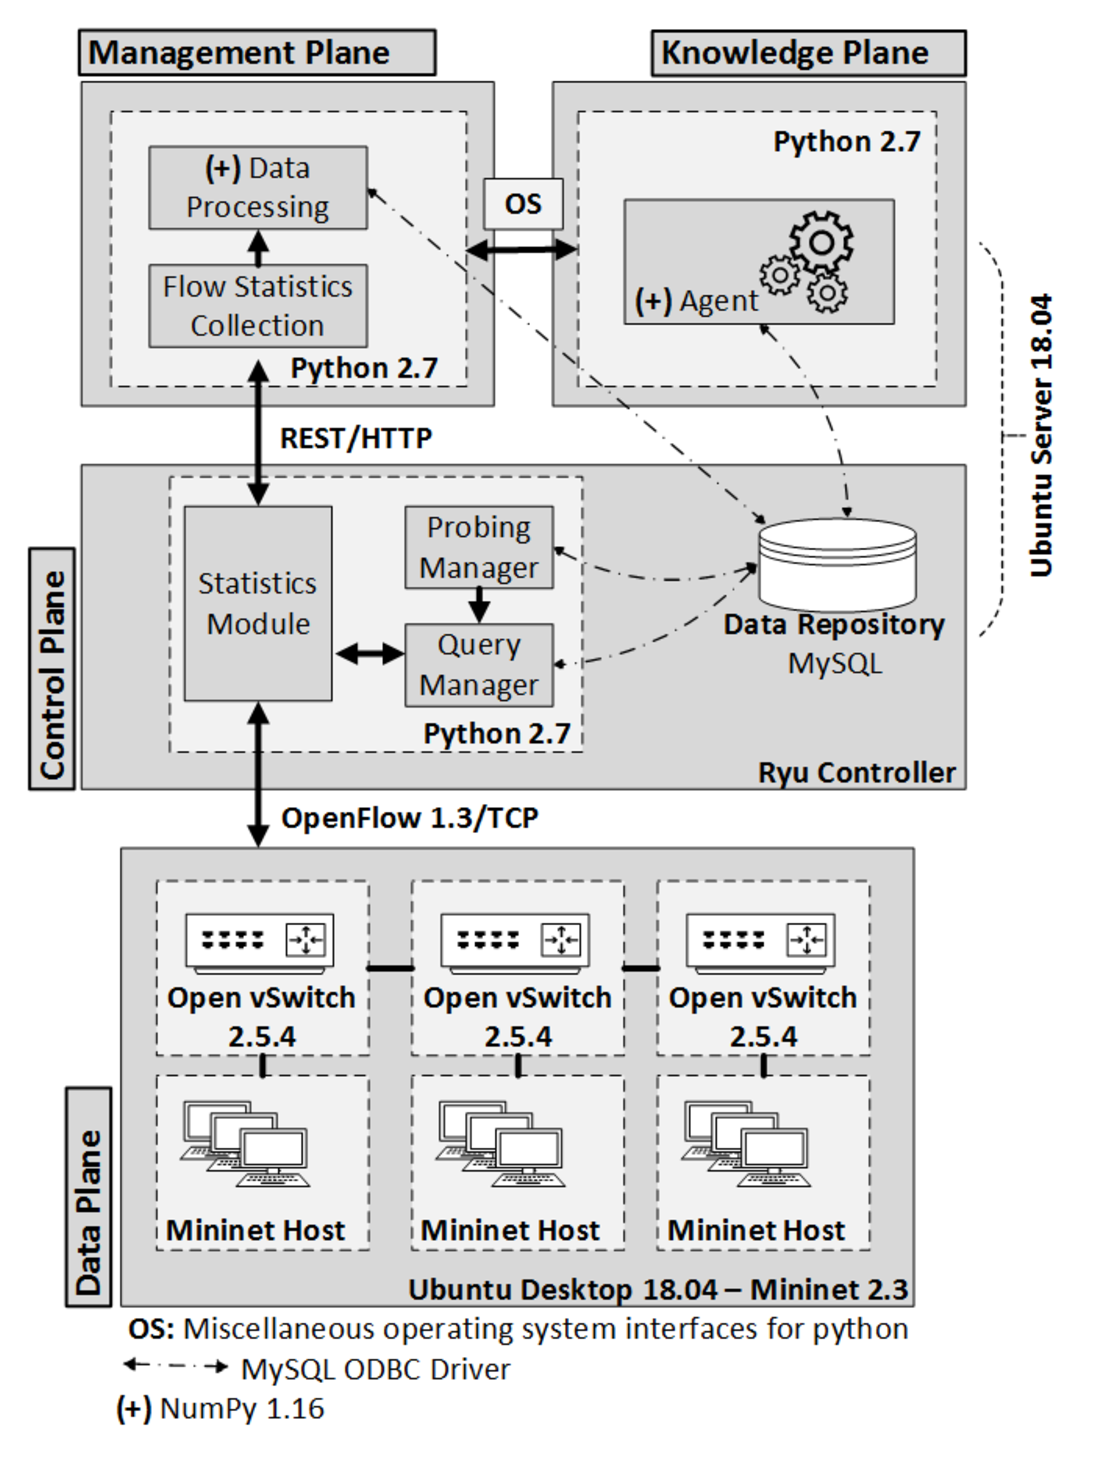
\includegraphics[scale=0.5]{figures/Fig5-IPro-prototype}
    \caption{IPro - Prototype}
    \label{fig:prototype_ipro}
\end{figure}

It is important to highlight that the \textit{Statistics Module} interacts with DP by the OpenFlow Protocol \cite{onf_2012:openflow}. This protocol was used because it has progressively turned on the SBI \textit{de-facto} standard in SDN \cite{nunes_2014:survey_past_present_future}. OpenFlow describes an open protocol that allows software applications to program (\textit{i.e.}, add, update, and delete flow entries) the flow table of the OpenFlow-compliant switches. In particular, the \textit{Statistics Module} uses the OpenFlow version 1.3. Specifically, this module uses two Read-State (Request-Reply) messages to collect information from the switch, such as current configuration, statistics, and capabilities. The controller sends a Read-State Request message to the switches to request the traffic statistics of flows. The switches communicate to the controller the requested traffic statistics via Read-State Reply messages. To get OpenFlow details,  the reader to Openflow specification is refered \cite{onf_2012:openflow}.

\subsection{Space of States}
\label{subsec:space_states}

To determine the finite space of states (\textit{cf}. Equation~\ref{equ:states_model}) that the IPro RL-agent needs to operate, first, the CCO (\textit{cf}. Equation~\ref{equ:load}), CUC (\textit{cf}. Equation~\ref{equ:load_cpu}), and MA (\textit{cf}. Equation~\ref{equ:ma}) were estimated and experimentally measured when the probing interval varies. The probing intervals between 1 and 15 seconds were manually tested (in steps of 1 second). For each interval, the test duration was 600 seconds. Second, the CCO and CUC were discretized by using the obtained results.

\subsubsection{Control Channel Overhead}
Aiming at determining the space of states that the IPro RL-agent needs to operate, Figure~\ref{fig:control_channel_load_behavior} presents the impact of the probing intervals on CCO. If the network is monitored with a probing interval upper or equal than 5 seconds, the overhead is lower than 12\%. When this interval is smaller than 5 seconds the overhead increases (top than 20\%) due to the big size and quantity of Read-State (Request-Reply) messages (\textit{cf}. Equation~\ref{equ:load}). These results corroborate that the probing interval affects CCO significantly.

\begin{figure}[h!]
    \centering
    \includegraphics[width=1.0\textwidth]{figures/Fig7-control-channel-behavior}
    \caption{CCO Variation}
    \label{fig:control_channel_load_behavior}
\end{figure}

\subsubsection{CPU Usage of the Controller}
Aiming at determining the space of states that the IPro RL-agent needs to operate, Figure~\ref{fig:cpu_behavior} presents the impact of the probing intervals on CUC. If the network is monitored with a probing interval upper or equal than 5 seconds, CUC increases on average 8.5\% approximately. Nevertheless, when this interval is smaller than 5 seconds, CUC increases (top than 20.5\%) because the controller collects statistics information more frequently. As a consequence, the controller CPU must process a higher amount of instructions per second for (de)fragmenting and reading the Read-State messages. Overall, these results corroborate that the probing interval can affect CUC significantly.

\begin{figure}[h!]
    \centering
    \includegraphics[width=1.0\columnwidth]{figures/Fig6-cpu-usage}
    \caption{CUC Variation}
    \label{fig:cpu_behavior}
\end{figure}

\subsubsection{Monitoring Accuracy}

\begin{figure}[h!]
    \centering
    \includegraphics[width=1.0\columnwidth]{figures/Fig9-throughput}
    \caption{MA of throughput }
    \label{fig:throughput}
\end{figure}

To evaluate MA, the throughput metric was measured in each probing interval and determine its respective accuracy using Equation~\ref{equ:ma}. Figure~\ref{fig:throughput} depicts the evaluation results, disclosing that MA in the throughput measured is higher than 80\% when the probing interval varies between 4 and 6 seconds. In particular, the interval of 5 seconds reports the highest MA (88.83\%). In turn, the intervals of 6 seconds and 4 seconds achieve an MA equal to 86.06\% and 83.83\%, respectively. Nonetheless, MA reduces considerably for the other probing intervals. For instance, the interval of 7 seconds accomplishes an MA lower than 69.93\% due to the reduction in the quantity of collected information. In turn, the probing intervals 1, 2, and 3 seconds lead to high CCO that interferes with SDN management messages. Furthermore, these intervals also lead to high CUC that compromises the correct operation of the controller and, so, of the underlying data plane. These two facts deteriorate the correct operation of the network generating high TCP errors and low processing of SDN management messages (\textit{cf}. Figure~\ref{fig:tcp-erros}). Therefore, the MA of data collected is also affected. In summary, the above results corroborate that the probing interval affects MA significantly.

\begin{figure}[h!]
    \centering
    \includegraphics[width=1.0\textwidth]{figures/Figure9b-tcp-errors}
    \caption{TCP errors generated by Monitoring Interference}
    \label{fig:tcp-erros}
\end{figure}

\subsubsection{Spaces Discretization}
Since IPro is RL-based, it models its environment as a finite MDP. In order to get a finite space of states, the CCO and CUC were discretized by using the results above presented (\textit{cf.} Figures~\ref{fig:control_channel_load_behavior} and ~\ref{fig:cpu_behavior}) as follows:

\begin{enumerate}
    \item The values of CCO and CUC are represented in the interval $\left [ 0,1 \right ]$, where 0 represents 0\% and 1 represents 100\%.
    \item The policy 1 (related to the threshold $\omega$) is set to 80\% aiming at preventing response times of controller upper than 1 millisecond \cite{repas_2015:performance_cpu}. Thus, \\
    CCO: $ l =\left \{ \left [ 0,0.4 \right ), \left [ 0.4,0.5 \right ), \left [ 0.5,0.6 \right ), \left [ 0.6,0.7 \right ) ,\left [ 0.7,0.8 \right )\right \}$.
    \item The policy 2 (related to the threshold $\chi$) is set to 80\% targeting to avoid interference with essential SDN functions (\textit{e.g.}, packet forwarding and route updating) and the reduction of network performance \cite{xu_2017:wildcard_requests}. Thus, \\
    CUC: $cpu=\left \{ \left [ 0,0.4 \right ),\left [ 0.4,0.5 \right ),\left [ 0.5,0.6 \right ),\left [ 0.6,0.7 \right ),\left [ 0.7,0.8 \right ) \right \}$.
    \item The Probing Interval: $i = \left \{\left [ 4,10 \right ] \right \}$. 
\end{enumerate}

It is important to highlight that CCO and CUC can be divided into smaller sub-intervals to facilitate the RL-agent decision making process. However, smaller intervals increase the size of the space of states and, so, slow down the learning process convergence rate. Thus, the discretized space of states is:

{\setlength{\mathindent}{3cm}
\begin{equation}
    \begin{split}
      S\equiv f\left ( i, l, cpu \right ): & i\in \left [ 4,10 \right ], l=\left \{ 0,0.4,0.5,0.6,0.7,0.8 \right \},\\ 
      & cpu=\left \{ 0,0.4,0.5,0.6,0.7,0.8 \right \} 
    \end{split}
    \label{equ:states}
\end{equation}
}